%!TEX root = ../main.tex

%FLUFF THE INTRO
\section{Modelling}
Modelling of a real world system has two motivators, the first is to gather better understanding of the system through mathematics and data analysis, the other is to facilitate the optimisation and simulation of the system. However there are challenges that can affect the accuracy of the model, as such careful deliberation should be taken to make good assumptions and simplifications. The assumptions and simplifications that are made will be explained and justified for each relevant algorithm, sub-model and constraint; all of which are needed to properly communicate the model in such a way that is independent of the optimisation techniques used.  
\\
The models defined in this section of the report will be used in all optimisation methods attempted, the accuracy of these models is vital to the accuracy of any formulation dependant on them and as such proper considerations and justifications must be made. The models that are discussed here are inherit to the system, they are often constants or functions within larger problem formulations, as such they are simple to change but yet key to the accuracy of the thesis. \\
The models discussed here are broken into four major sections:
\begin{itemize}
 \item Proper modelling of spoil distribution.
\item Modelling of movement patterns within a block.
\item Modelling of data unique to a dragline .
\item The modelling of an action.
\end{itemize} 
Each of these categories aligns with a specific section of a formulation, and as such can be developed independently of each other. 
\subsection{Spoil modelling}
The Spoil or overburden is the strictest constraint on the feasibly of a strip, as such the modelling of spoil distribution is vital to the accuracy of a model. The spoil channel can be discretised into sections with a given maximum capacity per section, following this the swell rate of the spoil and expansion factor due to inefficient spoil placement should also be considered. These three models are the required knowledge to properly consider and implement spoil capacity constraints on a formulation, each model can be seen below. 
\subsubsection{Spoil Capacity}
The capacity of a section of spoil is a vital constraint in the formulation of a block model, the capacity of the spoil is therefore modelled as the maximum amount of spoil that could stably be held at that section without collapse of the spoil channel, the stable angle for loose overburden to be stacked is 36 degree, with the spoil channel 20m lower than that of the mine therefore by using an approximate model of a cone to represent each spoil section, then the spoil capacity is $0.33\times W^2/2 \times H $ is the maximum spoil capacity. 
\subsubsection{Swell Factor}
Swell factor is the amount of expansion in volume for material being dumped into the spoil channel, the typical swell rate of of compact dirt can be modelled as an increase in volume of 30\% \cite{SpoilUtilization}. The modelling taken from prior resources such as textbooks is sufficient for the purposes of this thesis.
% \subsection{Movement through a Block}

	
% \subsection{Dragline Dynamics}

\subsection{Action Cost}
The cost of an action is here defined as the time taken to move overburden from a section in the mine to a section on the spoil, this should be based either on experimental data or through a  model of a dragline. However modelling the entire system proves difficult in one dimension, as a result the method suggested in section 3.1 was considered. The model is that  the time taken to move the dragline is a linear relationship with the angle that the dragline is moving \cite{Dmove}. \\The calculation of the angle is simple, the distance from the draglines current point to the point in the spoil can be found using basic trigonometry and as such the cost of an action is defined below. 

\section{Optimisation at the Block Level}
In order to model a sequence of blocks it is vital to first develop an accurate model describing the cost and spoil of a block. Several methods were considered, each of which was an optimisation problem seeking to minimise the time taken to process the block. The calculation and modelling of a block must be rapid, as this modelling function will be used thousands of times in the calculation of a strip, while storing block costs into memory was originally considered the feasibility and cost of a block varies with three inputs, its start and end locations, and the current state of the spoil. Therefore the amount of unique blocks that can be considered is huge and storing results in memory loses efficiency \\A variety of methods were formulated and the results were compared against one another for both run time and accuracy, in order to verify the accuracy of a model its output is compared to techniques that are outlined in section 3.2. This comparison was done on both real world data and standard data sets that were generated for the purpose of testing. The comparison will focus on the run times of each solution as well as the accuracy of the method proposed. 

\subsection{Mixed Integer Programming}
Mixed Integer Programming is a somewhat obvious choice for this model. This technique is  applied in a 3 dimensional environment as outlined in section 3.1, however some changes must be made for this model to be used with the modified density data. While the use of a MILP was still considered, the problem itself must  be reformulated. Formulation for the model is found in the following section, while developing a MILP it is vital that all constraints and objectives are linearly related to data and variables, otherwise the solver algorithms will not work \cite{gurobi}. The process of formulating an appropriate model for the block cost is based on the physical movements of a dragline and the constraints that will affect it, while some elements of the formulation were adjusted or ignored, the end formulation is the most accurate model for the data available. 
\subsubsection{Model Formulation} 
\paragraph*{Sets}
\begin{align}
\label{MIP:Set:S}
S\qquad \text{Set of all Spoil Sections   } s\in S\\
\label{MIP:Set:N}
N\qquad \text{Set  of all Mine Sections } m \in M
\end{align}
Here the sets are used to represent the discrete mine and spoil sections, these sets are used for communication and organisation  of data and variables. The sizes of sets $S$ and $M$ must be the same as the spoil channel is the results of a prior strip in a mine. The discretisation of the Mine into sections was chosen as the move from a continues model to a discrete model made the modelling of the problem much easier. While some information is lost in this process it is negligible as survey data itself is discrete.

 The size of the sections themselves are dependent on both survey data and desired accuracy, for the testing of this thesis each section was a metre in length, however if more precision is required,  the resolution could be increased. The increase in detail and resolution will result in slower calculations of block dimensions as more potential solutions are presented. One metre was selected because it was the resolution of the real world data supplied.
 % however as seen in the comparison of results a lower resolution will dramatically speed up the run time of the problem, this could be used in first pass solutions to get an approximation of good results. 
\paragraph*{Data}
\begin{align}
\label{MIP:Data:SF}
SF \qquad \text{Swell Factor of Spoil}\\
\label{MIP:Data:Seff}
SEf \qquad \text{Packing Efficiency of Overburden}\\
\label{MIP:Data:SpoilCap}
SpoilCap \qquad \text{Maximum capacity of spoil}\\
\label{MIP:Data:n}
n_{j} \qquad \text{Density of overburden at section $j$} \quad \forall m_{j}  \in M\\
\label{MIP:Data:s}
s_{j} \qquad \text{Density of overburden at section $j$} \quad \forall s_{j}  \in S\\
\label{MIP:Cost}
C_{jk} \qquad \text{Cost of movement from $m_{j}$ to $s_k$ }\\
\label{MIPDvol}
Dvol \qquad \text{Volume of overburden moved in one action}
\end{align}
The data relevant to the formulation of the MIP is modelled and calculated in section 4.1, in this section models and justifications can be made for each design choice that is made in the accuracy of the data however in this section the way that the data is used is much more important. The data used is relatively simple, often represented as either a constant or an array of constants. The use $SF$ (\ref{MIP:Data:SF}) to represent the swell of spoil is vital to the proper modelling of spoil distribution and will be used whenever interacting with the spoil output of the system, this data is simply a constant value, as suggested in the prior section. Similarly $SEf$ (\ref{MIP:Data:Seff}) is used as an approximate model for the expansion of the spoil due to inefficiencies in stacking methods, this constant can vary depending on the model used however is simply represented in the formulation of this problem and is not a key data point for initial testing, rather it is important for the accuracy of the spoil channel distribution, which itself is also dependant on $SpoilCap$ (\ref{MIP:Data:SpoilCap}) or the maximum capacity of the spoil at any given section $s$, here we assumes that this capacity is constant throughout the spoil channel, however this could be easily adapted if needed for varying capacities. This capacity is used in the constraint constricting the amount of spoil able to be dumped in a section (\ref{MIP:SPcap}) as the right hand side of the equation. Sensitivity analysis could be done on this constraint to estimate the potential benefits of increasing the capacity of spoil available, this would have the same effect as increasing the efficiency of the spoil stacking methods, as described by a lower value of $SEf$ (\ref{MIP:Data:Seff}).\\
The amount of material moved per action can be found in $Dvol$ (\ref{MIPDvol}), while a very simplistic piece of information it is still necessary to include as it represents the amount of overburden moved per action through the size of the draglines bucket. Sensitivity analysis could also be done to relate how the changing size of this constant affects the mining time of a block, increasing this constraint should reduce the cost of the block as it will reduce the amount of actions required to remove the overburden from a mine section. This cost is found in $C_{jk}$ (\ref{MIP:Cost}) however this data is an $m\times s$ array that contains the movement cost from each point $m\in M$ to each spoil section $s \in S$, the movement cost is used in the objective function to minimize the total swing time of the dragline inside a block. This cost data can be calculated as a function $\arctan(\frac{abs(n-s)}{Reach})$ however this may also be pre-calculated and put into an array to reduce function calls, the latter method was selected for the implementation of this data. 
\\
The representation of the mine\ref{MIP:Data:n} is an $1\times m$ array where the value at each point is the average amount of overburden to be removed at that point, this value will not change as we will never come back to or refer to a section once the overburden has been removed. Unlike this is data \ref{MIP:Data:s} which represents the amount of overburden currently in the spoil. Once a block is calculated this spoil value is updated so that future blocks use the spoil output of the previous block to have a consistent and proper model for the spoil distribution throughout the strip. Therefore while this data will not change during the calculations performed on the block, once the solution is calculated this data is updated to reflect on the resultant spoil. 
\paragraph*{Variables}
\begin{align}
\label{MIP:M2S}
X_{jk} \qquad \text{Overburden moved from $m_{j}$ to $s_k$ }\\
\label{MIP:MCeil}
Y_{jk} \qquad \text{Actions moving from $m_{j}$ to $s_k$ }
\end{align}
The variables for this model are both related to the movement of overburden from a mount $m$ in the mine to a point $s$ in the spoil. Variable $X_{jk}$ (\ref{MIP:M2S}) refers to the capacity of dragline volume that is moved from $m$ to $s$. This is necessary for the calculation of spoil capacity constraints as well as the calculation of removal of overburden from the mine at point $m$. However the assumption is made that movement actions taken at any capacity will still incur the same costs. It is for this reason that variable $Y_{jk}$ (\ref{MIP:MCeil}) is used, representing the ceiling of actions taken from point $m$ to point $s$ for all points in the mine. This variable is exclusively used in the objective function, participating only in constraints that allow it to be linked to \ref{MIP:M2S}.
\paragraph*{Objective}
\begin{align}
\label{MIP:OBJ}
\min\left(\sum_{m\in M}\sum_{s\in S} (C_{n,s}\times Y_{n,s})\right)
\end{align}
The objective function of the MILP is simple, the minimisation of time taken to complete all actions. As some actions will cost more than others it becomes obvious that the cheapest possible movement will be selected when available, it should be noted that while cost\ref{MIP:Cost} is not linear, its relationship with movement actions \ref{MIP:MCeil} is, allowing linear programming to be used. The minimization of this is obvious, as smaller movement actions will take less time than a larger swing action, they will be preferred where feasible. 
\paragraph*{Constraints}
\begin{align}
\label{MIP:RemoveAll}
\sum_{s}X_{m,s}\times Dvol = M_{m}  \quad \forall m\in M  \\
\label{MIP:SPcap}
\sum_{m\in M} X_{m,s}\times SEf \times SF + S_s\leq SpoilCap \quad \forall s \in S \\ 
\label{MIP:Link}
X_{m,s} \leq Y_{\mu,s} \quad \forall m,s \in M,S\\
\label{MIP:Housekeeping}
X_{m,s} \geq 0 \qquad \forall m \in M , s \in S\\
Y_{m,s} \in \mathbb{N} \qquad \forall m \in M , s \in S
\end{align}
The constraints on the model could be considered as the most interesting part of the model, with no constraints the model would simply choose to perform no actions, as this is the minimal allowable solution. Therefore the minimum amount of work done by the dragline must be constrained, the strict constraint found in  equation \ref{MIP:RemoveAll} states that all overburden must be removed from a section $m$ for all sections in the mine. The purpose of this constraint is to set the exact amount of overburden removed by the dragline, it must remove all overburden from the block, but cannot remove any additional material from the block, while the latter is less likely as this would increase the cost of operation it is still best to have as strict a constraint as possible. \\
The constraint described in equation \ref{MIP:SPcap} constrains the solution the most of any constraint in not only the block model but the entire thesis, it is the feasibility constraint that the spoil capacity cannot be exceeded, it should be noted that this constraint also takes into account the state of the spoil prior to this block, allowing past blocks actions to carry over. This constraint will invalidate many solutions and cause the cost of action to go up if all local spoil sections are at or close to capacity, this constraint is what drives up the cost in the calculation of a block. 
\\ Constraint \ref{MIP:Link} is the linking constraint between $X$ (\ref{MIP:M2S}) and $Y$ (\ref{MIP:MCeil}), it ensures that $Y$ is the ceiling of $X$. As the objective is a minimisation problem, then $Y$ will seek to be the lowest allowable integer value greater than or equal to $X$, this linking constraint ties constraints \ref{MIP:RemoveAll} and \ref{MIP:SPcap}, which are both dependent on $X$ to the objective function \ref{MIP:OBJ}, which is dependent on $Y$. Similarly constraints \ref{MIP:Housekeeping} simply state that $X$ must be a positive real number and $Y$ must be an integer greater than or equal to zero, these constraints are simply to properly set up the variables for the model. 
\subsubsection{Implementation}
The implementation of the model is done in Python, with use of the gurobi optimisation engine linear programming becomes very simple. The implementation of the model is such that the calculation and algorithms associated with linear programming are performed by the gurobi optimisation engine. As such the implementation is simply setting up the formulation in a way that the optimisation engine will understand.
\begin{lstlisting}[language=Python]
		m = G.Model() 
		X = {(n,s):m.addVar() for n in self.N for s in self.S}
		Y = {(n,s):m.addVar(vtype = G.GRB.INTEGER) for n in self.N for s in self.S}
		\end{lstlisting}
		This section of the code sets up the two variables $X_{jk}$ and $Y_{jk}$ such that X is a continuous variable and Y is constrained to be an integer. The dimensions of both X and Y are $M \times S$ as can be seen in the section \begin{lstlisting}for n in self.N for s in self.S\end{lstlisting} which is two for loops iterating over the entire mine. 
		\begin{lstlisting}[language=Python]
		m.setObjective(G.quicksum((self.MoveCost(n,s)*Y[n,s]) for n in self.N for s in self.S),G.GRB.MINIMIZE)
		\end{lstlisting}
Here the objective is declared and set to minimise , matching the objective \ref{MIP:OBJ} stated in the formulation section. This will minimise the cost of movement for each potential movement on the block, this must be considered only for the variable Y as it is the ceiling of X and is present in the mathematical formulation.	\begin{lstlisting}[language=Python]
		CreateCieling = {(n,s):X[n,s]<=Y[n,s] for n in self.N for s in self.S}

		RemoveOnlyallowed = {
		(n):m.addConstr(G.quicksum(X[n,s]*self.Dragline.get_BucketVol() for s in self.S)==self.Mine[n]) for n in self.N
		}

		spoilcapacity = {
		(s):m.addConstr(G.quicksum(X[n,s]*self.Dragline.get_BucketVol()*self.swell*self.expand for n in self.N)+self.Spoil[s]<=self.spoilcap)
		for s in self.S
		}

		m.optimize()
\end{lstlisting}
This section of code sets up the constraints similar to those outlined in the mathematical formulation with each constraint \ref{MIP:Link} ,\ref{MIP:SPcap} ,\ref{MIP:RemoveAll}  represented in code. For additional information on supporting code please refer to Appendix A. \\  Once the formulation is complete gurobi will perform preprocessing on a matrix representation of the model, before using the modified simplex algorithm to solve the linear problem\cite{gurobi} at each step the linear program is then branched to integer solutions, however as the integer section of the formulation is used to act as an upper bound on the continuous variable the branching operation is very efficient. 
Once this optimisation algorithm has been completed the spoil is updated and the cost is returned, this is done by simply updating the relevant sections of the array and can be seen completed in the below code snippet.
\begin{lstlisting}[language=python]
self.cost = m.ObjVal
self.potential_spoil = self.Spoil[:self.step]+[sum(M2S[n,s].x*\
self.Dragline.get_BucketVol()*self.swell*self.expand for n in self.N)+self.Spoil[s]\
 for s in self.S]+self.Spoil[self.etemp:]

\end{lstlisting}
This entire process is then wrapped into one function so that the cost of a block can be calculated though one function call, vital to the application of this model in the optimisation of the entire strip. 
\begin{lstlisting}[language=python]
	def BlockCost(self,start,end,Spoil,output=0):
		if end>len(self.Mine):
			end = len(self.Mine)
			# print("Adjusting End Position")
		self.set_Spoil(Spoil)
		if output ==1:
			print("Spoil Set")
		self.set_Block(start, end)
		if output ==1:
			print("Block Set:\t" ,[start,end])
		self.Calc_Valid()
		if output ==1:
			print("Column Generation Done")
		stime = time.time()
		try:
			self.MIP(output)
			etime = time.time()-stime

		except:
			etime = time.time()-stime
			print('\t MIP Infeasible')

			return(np.inf,Spoil,etime)
		if output ==1:
			print("MIP Complete")
		return (self.cost,self.potential_spoil,etime)
		\end{lstlisting}
The only unique or interesting part of this function is that if the block is not feasible then the function will return a cost of infinity, meaning that the block will not be used in the optimal or feasible solution of a sequence of blocks in a strip. Each call of the function take in the start, end and state of the spoil, allowing the block to be calculated to return the cost and updated spoil, as well as the time taken to calculate the MIP. Both cost and resulting spoil are vital to the calculation of the strip, and are the two desired outputs of any model describing the actions taken within a block. 
\subsubsection{Results of MILP formulation}
A set of 10 generated cases were selected for comparing the presented algorithms and models against each other, the first five cases are on an open spoil and increase in complexity, the final five cases have spoil channels of increasing complexity. Where possible the results of potential blocks captured in the same locations of each mine are considered. In this section of results, prior to comparison to other such methods the type of solution received will be inspected.	It should be noted that Dataset 1 is the real world data supplied and all other data types are generated for the purposes of additional testing. 
\begin{figure}[h]
\label{MIP1-1}
\caption{Block Analysis for real world Data}
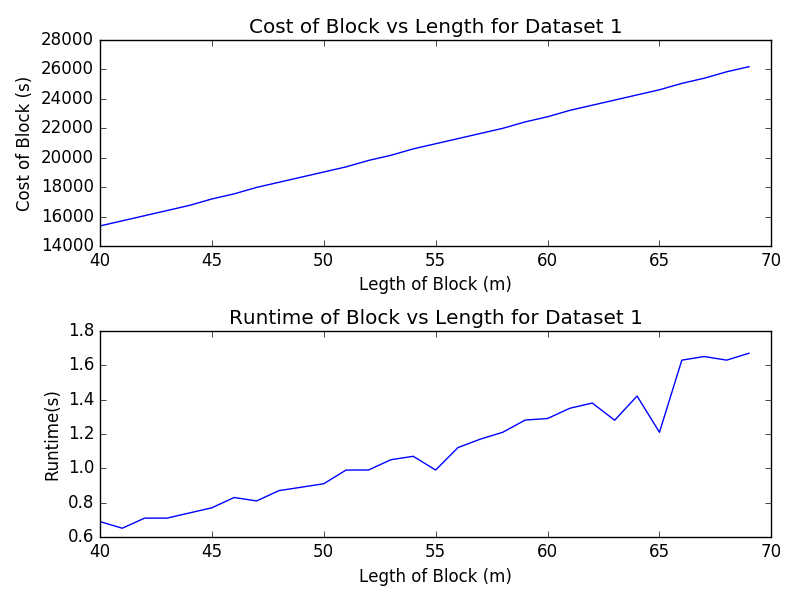
\includegraphics[width=\textwidth]{MILP1_D1.png}
% \label{MIP1-2}
% 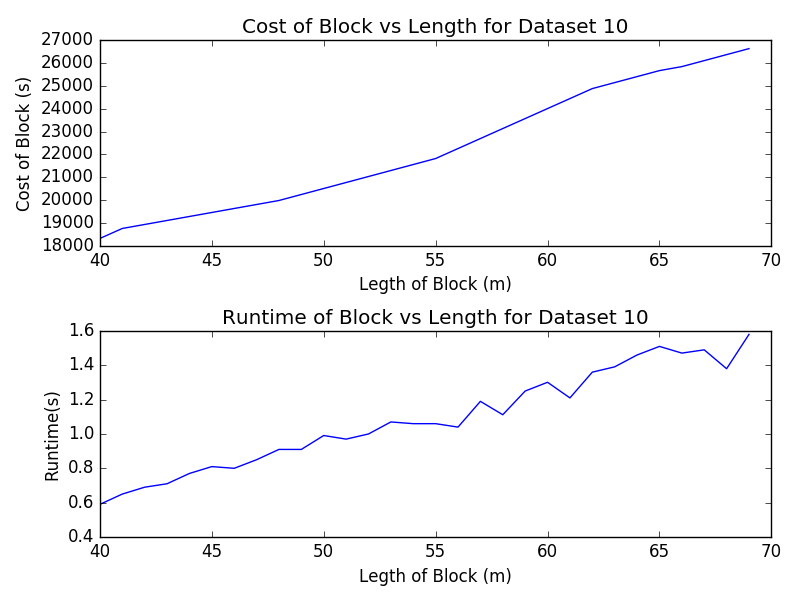
\includegraphics[width=\textwidth]{MILP1_D10.png}
\end{figure}
The above figure \ref{MIP1-1} shows that the block is piecewise linear when calculated on an open spoil, that is the blocks cost can be represented as a series of linear functions which may appropriately approximate the block, this interestingly could be used as a potential alternative to the solution of a MIP problem. However the block will consistently increase in cost as the length increases, similarly as the size of the block increases as does the time taken to calculate and simulate its values. As can be seen in  figure \ref{MIP1-7} the dragline behaviour is similar although the cost will plateau at some points given the additional constraints of the spoil. This result suggests that while the cost of a block is linear under no or weak constraints any linearisation or simplification would not hold for blocks of more constrained or complex spoil channels. Therefore the use of a mixed integer linear program is still the best approach as it is capable of calculating the cost of a block rapidly and ensuring an accurate and optimal solution to the cost of a block. 

\begin{figure}[h!]
\label{MIP1-7}
\caption{Block Analysis for generated Data}
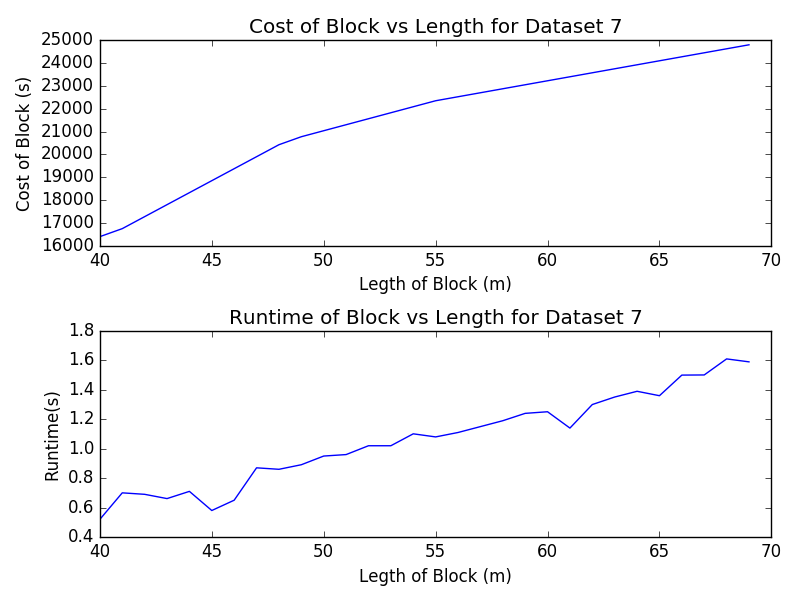
\includegraphics[width=\textwidth]{MILP1_D7.png}
% \label{MIP1-2}
% 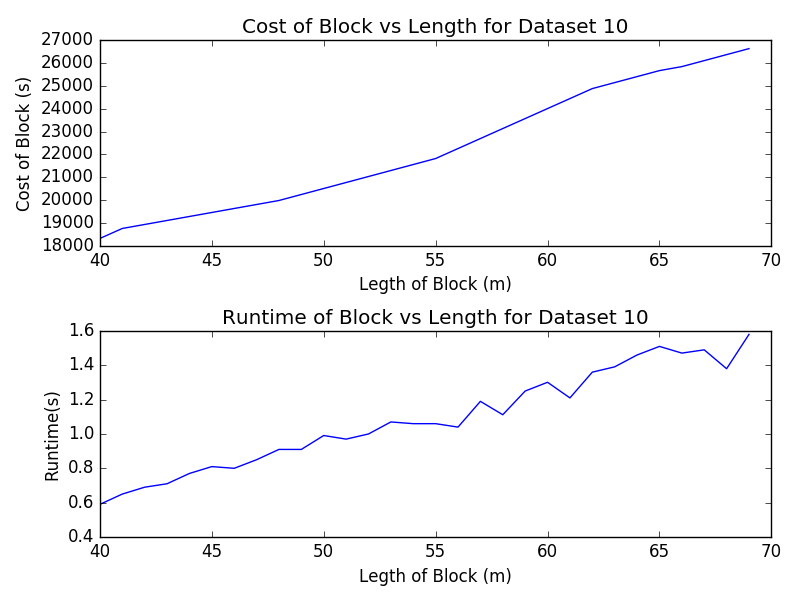
\includegraphics[width=\textwidth]{MILP1_D10.png}
\end{figure}
The typical increase in the cost of a block can be dependent on both the length of the block and the state of the spoil, however in this formulation the reach of the dragline is not properly considered. While this is acceptable for data sets with no or weak spoil constraints it will not function properly for more constrained blocks as the current model will incur a large cost to generate an infeasible solution where the suggested spoil section used is outside the reach of the dragline. 
\subsection{Mixed Integer Programming with Reachability Constraints}
This model is an updated version of the Mixed Integer model with only one added array of data and one additional constraint, however this single constraint makes a huge differences to the complexity and accuracy of the model. The constraint that a dragline cannot move to or reach every point in a block or in the spoil will constraint the areas where overburden can be distributed in the spoil section. This constraint was not initially obvious as typically the dragline will place spoil in local areas rather than in sections that would be out of its reach. However as the availability of spoil room is reduced the cost associated with this action is seen as preferable rather than an infeasible solution. This was only found after an implementation of the strip optimisation was complete, and as such can be seen as an updated model. 
\subsubsection{Model Formulation}
\paragraph*{Additional Data}

\begin{align}
\label{MIP:Data Valid}
Z_{jk}  = \begin{cases} 1& \text{if movement from $n$ to $s$ is reachable}\\
0 & \text{Otherwise}   \end{cases} 
\quad \forall n \in N s\in S
\end{align}
This data is an $m\times s$ array of binary values, such that if the dragline is able to feasibly reach the section of spoil when mining the section $m$ of overburden then the arrays value is 1 and 0 otherwise. This array is currently based on the feasible  maximum and minimum reach of the dragline, however other factors such as the pit edge while starting a new block, or having to move over sections in the spoil may cause this array to become more complex. Updating and improving this data should be of high importance for an accurate model, however as it is not integral to how the algorithm works, some simplifications can be made.
\paragraph*{Additional Constraints}
\begin{align}
\label{MIP:Valid}
Y_{n,s}\leq \infty\times Z_{n,s} \qquad \forall n \in N , s\in S
\end{align}
This constraint is a big M constraint, that is it will limit the value of Y unless the value of Z is one for that combination of m and s. This constraint is simply implemented and constrains the feasible solutions of the model, it should be noted that this is setting most of the potential values of Y and X before any optimisation is considered, doing this has a dramatic effect on the reduction of runtime. As less options are available, less calculations must be considered and as such the program can run faster.
\subsubsection{Implementation}
The code for this section is the exact same as previously, however one additional constraint is added, as can be seen below it is very simple to add additional constraints into the gurobi model.
\begin{lstlisting}[language=python]

OnlyifValid = {
		(n,s):m.addConstr(Y[n,s]<= np.inf*self.isValid[n-self.start,s-self.start-self.Dragline.get_reach()]) for n in self.N for s in self.S
		}
\end{lstlisting}
However more interestingly is the calculation of reachable blocks, as mentioned previously, the simplistic model for a reachable block is if it is within the reach of the dragline, while this is not an accurate model it is sufficient for the demonstration of the block planning algorithm and with more time could be developed to be more fitting for application. 
\begin{lstlisting}[language = python]
def Calc_Valid(self):
	self.isValid = np.zeros((self.end-self.start+1,self.end-self.start+2*self.Dragline.get_reach()+1))
	for i in range(self.end-self.start):
		for j in range(i-self.Dragline.get_reach(),i+self.Dragline.get_reach()):
			self.isValid[i,j+self.Dragline.get_reach()] = 1
\end{lstlisting}
Here the array size is set up, we only consider areas within the block and spoil and as such this will reduce the size of the array and allow for more rapid calculation of results. Once this is done for every possible combination of blocks in this window a check is done to ensure that it is a valid movement. 
\subsubsection{Results of Reachability formulation }
The results of the real world data should be the same as that of the prior formulation, this is because the additional constraint will only typically be applied when the spoil channel is crowded and potential solutions are restricted. When not in this situation the spoil will be placed in the lowest cost location possible, which is typically within the reach of the dragline. Despite the exact same cost for the block throughout this dataset the time taken per calculation is increased, this is due to both the additional constraint and the need to calculate the set of reachable positions for each location. This increased runtime suggests that a combination of both techniques could be valid, using the faster method on open spoil and the slower on a more constrained system. 
\begin{figure}[h]
\caption{Block cost comparison on an empty spoil}
\label{MIP-1}
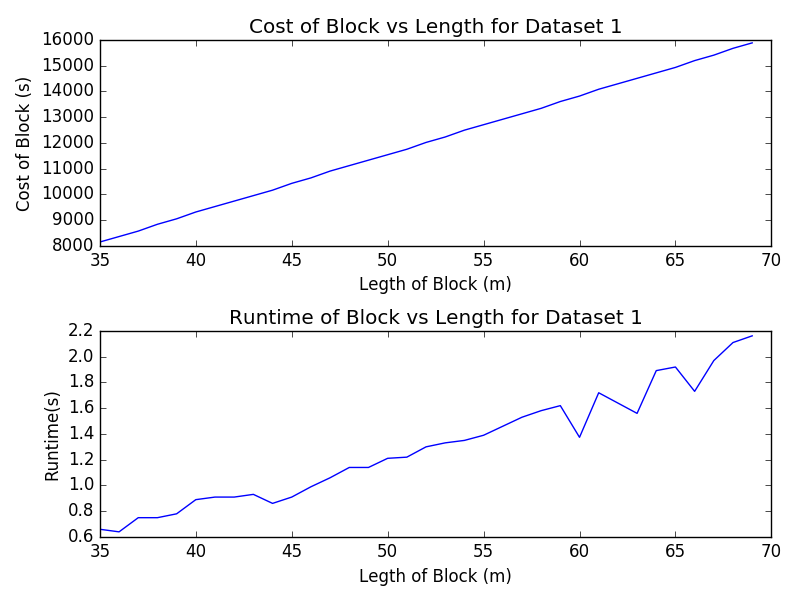
\includegraphics[width=\textwidth]{MILP2_D1.png}
\end{figure}
The results suggested in figure \ref{mip2dp7} suggest different solutions to those provided in figure \ref{MIP1-2}, this is due to the proper consideration of spoil location and capacity as well as the added constraint on reachability causes the cost of the block to be more expensive. Additionally this will have a differing spoil to that of the prior model and the individual actions may be drastically different. This model is more robust as it works in a constrained or under constrained environment. However other formulation methods should be considered as the run time of a block increases with both the complexity and the length of the block. 
\subsection{Dynamic Programming}
Dynamic programming is an obvious approach to the problem, as the use of memeotisation will decrease the amount of calculations required to find the optimal solution, unlike a MIP the dynamic program will recursively consider all potential solutions which while thorough could be sufficiently fast for the purposes of block cost optimisation. 
\subsubsection{Model Formulation}
\paragraph*{States}
\begin{align}
\label{Stte}
S \quad \text{State of spoil at current stage}
\end{align}
The state of a formulation is the current resources of remaining in a resource constrained dynamic program. Here this is the spoil channel, which will change with every action and therefore is updated at every stage, this state alongside the current stage should be stored in the memory so that the process of memotisation can occur. This technique uses the principle of optimality to reduce the amount of calculations required, that is if we have already calculated the optimal path for the block from this stage with the current states then the solution is already known and that branch of exploration can be completed. However the only state in this formulation is the amount of spoil in each section at the current stage, the use of this state is vital as it is used for the constraint on the actions available at each point. The spoil is a state as it will change with each action, nothing else will change depending on the action taken and therefore all other dynamic variables are simply stages. 
\paragraph*{Stages}
\begin{align}
\label{DP:Stage0}
H \quad \text{Overburden remaining at current block}\\
\label{DP:Stage1}
M \quad \text{current mine section }m \\ 
\label{DP:stage2}
D \quad \text{Position Of Dragline}
\end{align}
The stages of the model are something that we do not have control over, each action moves us from one stage to the next. This formulations two stages are interlinked, however it could also be seen that the position of the dragline is dependent on the current mine section. Therefore the model has effectively two stages, the overburden left at the current section and the current section within the mine. Once all overburden is removed from the stage $H$ the position $M$ is updated. If the position is sufficiently updated then the draglines position also will update. For any given block these stages will occur in the same order no matter what. This is the differentiation between states and stages, the dragline will always move through the block and remove all overburden however the actions taken to remove the overburden will not always be the same. Here the states are selected as the minimum required representation of the block in order to properly model its behaviors and movement process. 	
\paragraph*{Transition Function}
\begin{align}
\label{Transition}
S_{stage+1}(s)=S_{stage+1}(s)\times SEf  \text{where $s$ is the spoil section in action }
\end{align}
The transition value allows the next state to be calculated based on the current state and the action chosen. Here the action chosen is the moment of overburden from the current block to some point on the spoil $s$, this action will succeed in adding additional overburden to the relevant section on the spoil, updating this is simple and from here the only additional piece of information required is the constraint that this transition function cannot create a state that exceeds the spoil capacity, this is done by simply checking the suggested next state and adding a large cost if this constraint is violated. 
\paragraph*{Value Function}
\begin{align}
\label{value}
C_A = \arctan(\frac{abs(D-A)}{Reach})\\
V_t(S_t) = \min (C_A+V_t(S_{t+A}))
\end{align}
The value function calculates the cost associated with a given action based on the cost of the action and the resulting states for all future stages, the cost of an action is simply the swing time from the current block to the spoil selected as an action. This cost is to be minimised however will also affect the state of the next action, as such this will recursively consider all potential courses of action for each action taken. Therefore the more actions that can be made the more computation time is required to calculate the cost of a block. 
\subsubsection{Implementation}
The algorithm mentioned is performed recursively, at each iteration the position of the dragline and current block are updated, as they are stages they are very simple to update. Then the memory is checked to see if a solution already exists for this point. The process taken is simply outlined by the formulation above, but with minor changes to input saturation to take into account any limits on the system.
\begin{lstlisting}[language=python]
_Bucket ={}
M = MineGen(100)
S = [0 for i in range(130)]

def Bucket(Cur,End,SP,M,Scoops,H,D-):
    global _Bucket
    SPtup = str(SP)
    SPmax = 150
    Reach = range(D-20,D+20) 
    if D < 20:
        Reach=range(0,D+20) 
    if D-Cur<=5:
        D = D+5
    if H <=0:
        Cur = Cur+1
        Scoops = 0
        H = M[Cur]
    if Cur == End:
        return (0,0,0,0,[],0)
    if (Cur,End,Scoops,SPtup) not in _Bucket:
        _Bucket[Cur,End,Scoops,SPtup] = min((costspoilNL(Cur,A,H,D)+
            Bucket(Cur,End,SP[:A]+[SP[A]+28]+SP[A+1:],M,Scoops+1,H-10,D)[0],Cur\
                  ,A,Scoops,SP[:A]+[SP[A]+28]+SP[A+1:],D)for A in Reach if\
    SP[A]+28 <= SPmax)
    return _Bucket[Cur,End,Scoops,SPtup]

def GetData(Start,End,Mine,Spoil):
    try:
        A = Bucket(Start,End,Spoil,Mine,0,Mine[0],Start+20)
        Cost = A[0]        
        print("New Spoil Aquired")
        Flag = True
        NewSpoil = _Bucket[max(_Bucket.keys())][4]
        Position = A[5]
        print("Cost Of Block:",A[0])
    except:
        print("Failed")
        Flag = False
        Cost = 100000000000000
        NewSpoil = Spoil
        Position = 0
    return(Cost,NewSpoil,Flag,Position)

\end{lstlisting}
However in the memeotisation it is vital to include the state of the spoil, unfortunately this is likely to be unique and as such will not occur very often, this reduces the amount of memory calls made and the runtime of the program will increase, however if the state is not in the memory then the optimal solution of the problem has no guarantee to be returned, and instead a feasible solution will be supplied. 

\subsubsection{Results of Dynamic Program }
The cost of a block for real world data does not match the results suggested by the prior two methods as outlined in section 6.1, this is due to the incorrect use of memotisation will mean that optimal solutions cannot be found and the solutions supplied are feasible at best, however it should be noted that this formulation will generate the cost of a block drastically quicker than the two prior models, however the assumption can be made that any small saving in code time is negated by the huge loss in time taken to mine the block and other inefficient planning. 
\begin{figure}[h]
\caption{Block analysis on real world data }
\label{DP1}
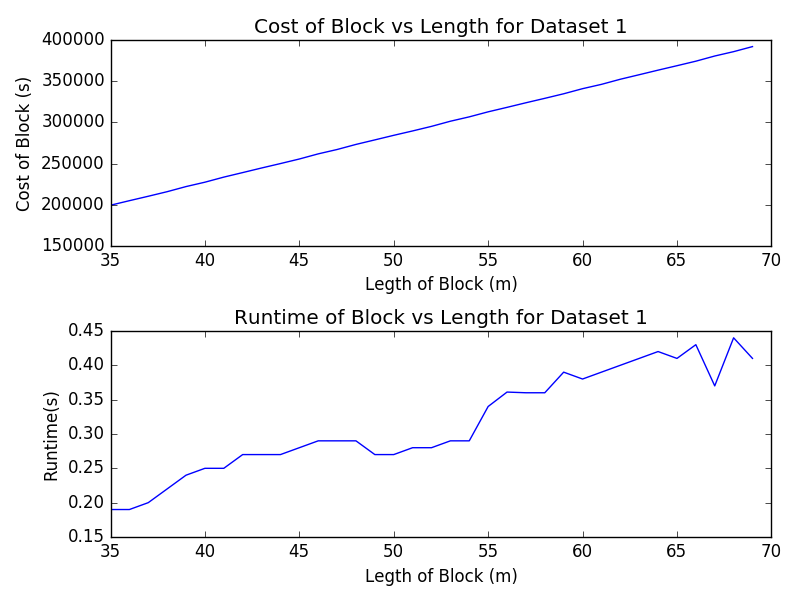
\includegraphics[width=\textwidth]{DP_D1.png}
\end{figure}
However when the state of the spoil was introduced to the memotisation, the run time of the solution increased massively, a hard timeout of 5 minutes was applied and no solution was found, further investigation showed that in five minutes A function call was performed $10^7$ times. This amount of function calls implies that the uniqueness of the spoil will limit the usability of the memotisation, and in fact only 8\% of those function calls were able to be avoided due to memotisation. This presents the problem that the optimal solution will take too long to calculate yet the feasible solution is incredibly fast to calculate. The poor performance of the dynamic programming technique is due in no small part to both the huge amount of possibilities but also the uniqueness of the states, the combination of these two factors suggests that the approach may not be appropriate for this problem, however some of the methods used here could be refined for other more fitting areas of the implementation.  
% \subsection{Comparison of Techniques}

\section{Optimisation of the Strip}
% \subsection{Mixed Integer Programming}
% \subsection{Mixed Integer Programming with Sequence Generation}
% \subsection{Dynamic Programming}
\subsection{Resource Constrained Dynamic Programming}
Resource constrained dynamic programming is a fitting solution to the optimisation of the strip, as the mine is explored blocks in a valid range are considered and the current position is updated. The amount of blocks required is not known in advance and therefore a resource constrained dynamic program will find all feasible solutions to this problem alongside the optimal solution. 
\subsubsection{Model Formulation}
\paragraph*{States}
\begin{align}
\label{Stte}
S \quad \text{State of spoil at current stage}
\end{align}
Similarly to the formulation of the cost of a block the spoil capacity at any point is the resource constraining the solution, this is fed into the block cost algorithm in order to properly obtain the optimal solution to the problem, as the spoil is updated creating blocks will become more difficult 
\paragraph*{Stages}
\begin{align}
\label{DP:Stage0}
M \quad \text{current mine section }m 
\end{align}
The stages of the model are something that we do not have control over, each action moves us from one stage to the next. This formulation is the current location of the start of the next block in the model, we consider this as a way of finding our end condition , however the stage is dependent on the actions taken prior, a longer block will result in a stage further on in the mine than usual. The use of a location as a state is vital to the understanding of the formulation. 
\paragraph*{Transition Function}
\begin{align}
\label{Transition}
S_{stage+1}(s)=S_{stage+1}(s)\times SEf  \text{where $s$ is the spoil section in action }
\end{align}
The transition value allows the next state to be calculated based on the current state and the action chosen. Here the action chosen is the movement of overburden from the current block to some point on the spoil $s$, this action will succeed in adding additional overburden to the relevant section on the spoil, updating this is simple and from here the only additional piece of information required is the constraint that this transition function cannot create a state that exceeds the spoil capacity, this is done by simply checking the suggested next state and adding a large cost if this constraint is violated. 
\paragraph*{Value Function}
\begin{align}
\label{value}
C_A = \text{Cost of block length A}\\
V_t(S_t) = \min (C_A+V_t(S_{t+A}))
\end{align}
The value function calculates the cost associated with a given action based on the cost of the action and the resulting states for all future stages, the cost of an action is simply the swing time from the current block to the spoil selected as an action. This cost is to be minimised however will also affect the state of the next action, as such this will recursively consider all potential courses of action for each action taken. Therefore the more actions that can be made the more computation time is required to calculate the cost of a block. 
\subsubsection{Implementation}
\begin{lstlisting}[language = python]
	def DP(self,position,end,spoil):
		self.count +=1
		print("Resource Constrained Dynamic Program \t Called:\t",self.count,'  times')
		print("Distance Remainging  :\t" ,end-position)
		if position>end-self.Dragline.get_minBlock():
			position = end
			# print("FUCK")
			return (10000000000000000000000000,0,[])

		if position == end:
			# print(value, sep, end, file, flush)
			return (0,0,[])
		# if end <= position:
			# self.dict[position,end,str(spoil)] = 100000000
			# return self.dict[position,end,str(spoil)]
		if (position,end,str(spoil)) not in self.dict:
			self.dict[position,end,str(spoil)] = min((10000+self.Blk.BlockCost(position,position+Action,spoil)[0]+
				self.DP(position+Action,end,self.Blk.BlockCost(position,position+Action,spoil)[1])[0]
				,Action,self.Blk.BlockCost(position,position+Action,spoil)[1])
			for Action in range(self.Dragline.get_minBlock(),self.Dragline.get_maxBlock()))
		return self.dict[position,end,str(spoil)]

\end{lstlisting}
\subsection{Resource Constrained Dynamic Programming with Sequence Generation}
The strongest constraint in the formulation of the strip is that the sum of all blocks must be equal to the length of the strip, that is $\sum B = L_s$. However in the prior formulation this constraint is not considered, this constraint is applied by generating all sequences of potential blocks that will equal the length of the mine as seen in the recursive function below. This set of potential solutions is much less than the potential solutions without this constraint and therefore the application of such a constraint will reduce the exploration of the dynamic program, sequence generation is done recursively as seen in the below code snippet. 
\begin{lstlisting}[language = python]
def GenBranchs(self,current,end,min,max,past):
	# count = count+1
	# print(count)
		if current == end :
			past+''
			self.Prunedstr.append(past)
			past = ''
			return 1
		if current>end:
			past = ''
			return -1
		for i in range(min,max):
			pred = past + ','+str(i)
			self.GenBranchs(current+i, end, min, max,pred)
		return 0
\end{lstlisting}
Once this is complete the potential solutions are a set of unique solutions to the problem, from here each potential solution is considered by using a forward dynamic program as formulated in the prior section, this modified method is seen below. 
\begin{lstlisting}[language = python]
def PrunedCost(self):
		self.best = np.inf
		self.bestStr = []
		counter = 0
		Flagg = 0
		for solution in tqdm(self.Prunelst):
			# counter+=1
			# print('Percent Complete:\t',counter/len(self.Prunelst)*100,'%')
			for Block in range(len(solution)):
				position = sum([solution[i] for i in range(Block)])
				# print(position,Block,solution)
				combo = ''
				if Block > 0:
					combo = str([solution[i] for i in range(Block)])
				if combo in self.prunedict:
					oldspoil = self.prunedict[combo][1]
					blockcalc = self.Blk.BlockCost(position,position+solution[Block],oldspoil)
					cost = self.prunedict[combo][0]+blockcalc[0]+10000
					# if cost > self.best:
						# Flagg = 1
						# break
				else:
					oldspoil = self.Spoil
					blockcalc = self.Blk.BlockCost(position,position+solution[Block],oldspoil)
					cost = blockcalc[0]+10000
					# if cost > self.best:
						# Flagg = 1
						# break
				newcombo = str([solution[i] for i in range(Block)])
				self.prunedict[newcombo] = [cost,blockcalc[1]]
			self.Prunefinal[str(solution)] = self.prunedict[str([solution[i] for i in range(Block)])]

\end{lstlisting}
% \subsection{Comparison of Techniques}
\subsubsection{Summary}
The implementation of the dynamic program without any preprocessing of potential solutions was unable to reach any final solution for a mine of length 500m, the result of this attempt was a five hour long simulation in which $10^{16}$ state combinations were explored before the program caused the computer to crash, this was found to be a reoccurring problem and was a key motivator for a method to reduce the amount of potential solutions considered. \\
Most solutions to the formulation can overshoot the problem by one block or undershoot it by less than one block, the set of solutions that can exactly equal the length of the mine is a small subset of the total solution space. The set of these sequences was generated and for a 500m strip was found to contain $10^9$ unique solutions to the problem. However the runtime of this sequence generation is $O(2^n)$ where n is the set of possible lengths the block could be. This runtime is not ideal for high resolution data however when compared to the previous method a solution is still found within three hours. The time taken to generate all possible sequences for a strip of 500m at a resolution of 1m is 900 seconds, however at a resolution of only 5m this is reduced to 200 seconds and $10^6$ solutions. Therefore a quick solution could be used as a heuristic for potential better solutions to reduce the amount of time taken. The time spent in the dynamic program however is still dramatically reduced as the runtime of the program is $O(|A|S^2|)$ and as the state space is reduced by a magnitude of 7 the states processed is also hugely reduced. 




